\documentclass[a4paper, 12pt] {article}

\usepackage[T1]{fontenc}
\usepackage{paralist}
\usepackage{amsmath}
\usepackage{romannum}
\usepackage{graphicx}

\graphicspath{{./images/}}
\newcommand{\head}[1]{\textnormal{\textbf{#1}}}

\begin{document}

\title{ECON-102: Principals of Microeconomics}
\author{Luka Trikha}
\maketitle

\section{Unit 1: Fundamental Concepts}
\subsection{Section 1: Economics}
In general terms, economics is defined as the study of how we can best increase
a nation's standard of living and citizens' happiness with the resources that we
have available to us.\\[2mm]
Standards of living include:
\begin{itemize}
    \item cars
    \item houses
    \item leisure time
    \item access to health care
    \item cleaner air
\end{itemize}

\subsubsection{Marginal Benefit \& Marginal Cost}
Marginal benefit and marginal cost can be though of as a positive cause-and-effect
in a business environment, with the benefit being the effect and cost being the
cause. When your marginal benefit is greater the marginal cost, the more likely
a positive investment is at play. For example, you may buy an expensive car for
your long commute, but it has the best MPG in the current car market and is 
heavily relaiable (maringal benefit)--potentially outweighing the initial cost
(marginal cost).

\subsubsection{Difference between Macro- \& Micro- economics}
Macroeconomics focuses on the wider concepts that play a role on the entire
economy. Components of this include:
\begin{itemize}
    \item national unemployment rate
    \item inflation rate
    \item interest rate
    \item federal government budgets \& fiscal policies
    \item economic growth
    \item Federal Reserve System \& monetary policy
    \item foreign exchange rates
    \item balance of payments
\end{itemize}
Microeconomics deals with the smaller concepts of an economy such as:
\begin{itemize}
    \item supply and demand of individual goods and services
    \item price elasticity (sensitivity) of goods and services in demand
    \item production
    \item cost functions
    \item business behavior and profit maximization
    \item income inequality \& distribution
    \item effects of protectionism (tarrifs, quotas, trade restrictions, etc.)
\end{itemize}
If macroeconomics is studying a forest, microeconomics is studying the
individual trees.

\subsection{Section 2: The Production Possibilities Curve}
\subsubsection{Production Choices}
Production choices are the idea that if you have limited resources to produces
various products, you want to optimize the resources at hand so that you can make
the most of the available resources, not underuse, and not over-promise a production
value that is not achievable.

\subsubsection{Points on the Curve and Trade-Offs}
In a given graph, any values that lie on the curve means that the operating cost
of the products are being used as efficiently as possible. The idea is that the
output cannot increase if it is limited by a constant resource and technology.
Scarcity talks about the limited resources at hand--which directly correlates
with the Production Possibility Curve. If a value lands on the curve, increasing
the production of one good/category will be at the expense of other goods/categories.
Points E, C, B, A, and D depicted in firgure \ref{fig:GnR1} represents the most
optimized products that can be produced with resources at hand. It also shows
varying priorities for both Guns and Roses productions.

Any points that fall inside the curve (to the left of the curve, i.e point G in
figure \ref{fig:GnR1}) shows an inefficent use of resources to produce products.
Some reasons for this could be using fewer than the available resources
(unemployment), or using all resources but inefficiently (underemployment).

Points that fall outside the curve (to the right of the curve, i.e point G in
figure \ref{fig:GnR1}) shows a combination that cannot be achieved with the
available resources. This value does not mean point F will never be achievable--
the economy may grow and F may fall on or inside the Possibility curve, but at
the current analysis of the economy, it will not be possible.
Increases in technology and/or resources can help contribute to the growth of
the Production Probability Curve, which can help reach point F in the future.

\begin{figure}[b]
    \centering
    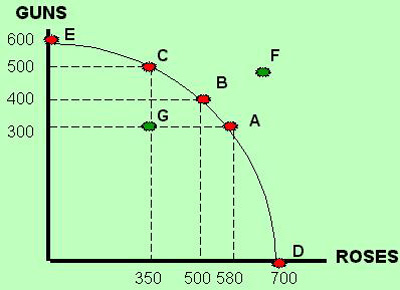
\includegraphics[width=5cm, height=5cm]{Production_Possibility_Curve.jpg}
    \caption{Example of a Possibility Curve of Guns and Roses production}
    \label{fig:GnR1}
\end{figure}

\end{document}
